\documentclass{article}
\usepackage[
    paperwidth=8.0139in,
    paperheight=6.2739in,
    margin=0in
]{geometry}
\usepackage[T1]{fontenc}
\usepackage[utf8]{inputenc}
\usepackage{newtxtext,newtxmath}
\usepackage{tikz}
\usetikzlibrary{arrows.meta,calc,positioning}
\pagestyle{empty}

\begin{document}
    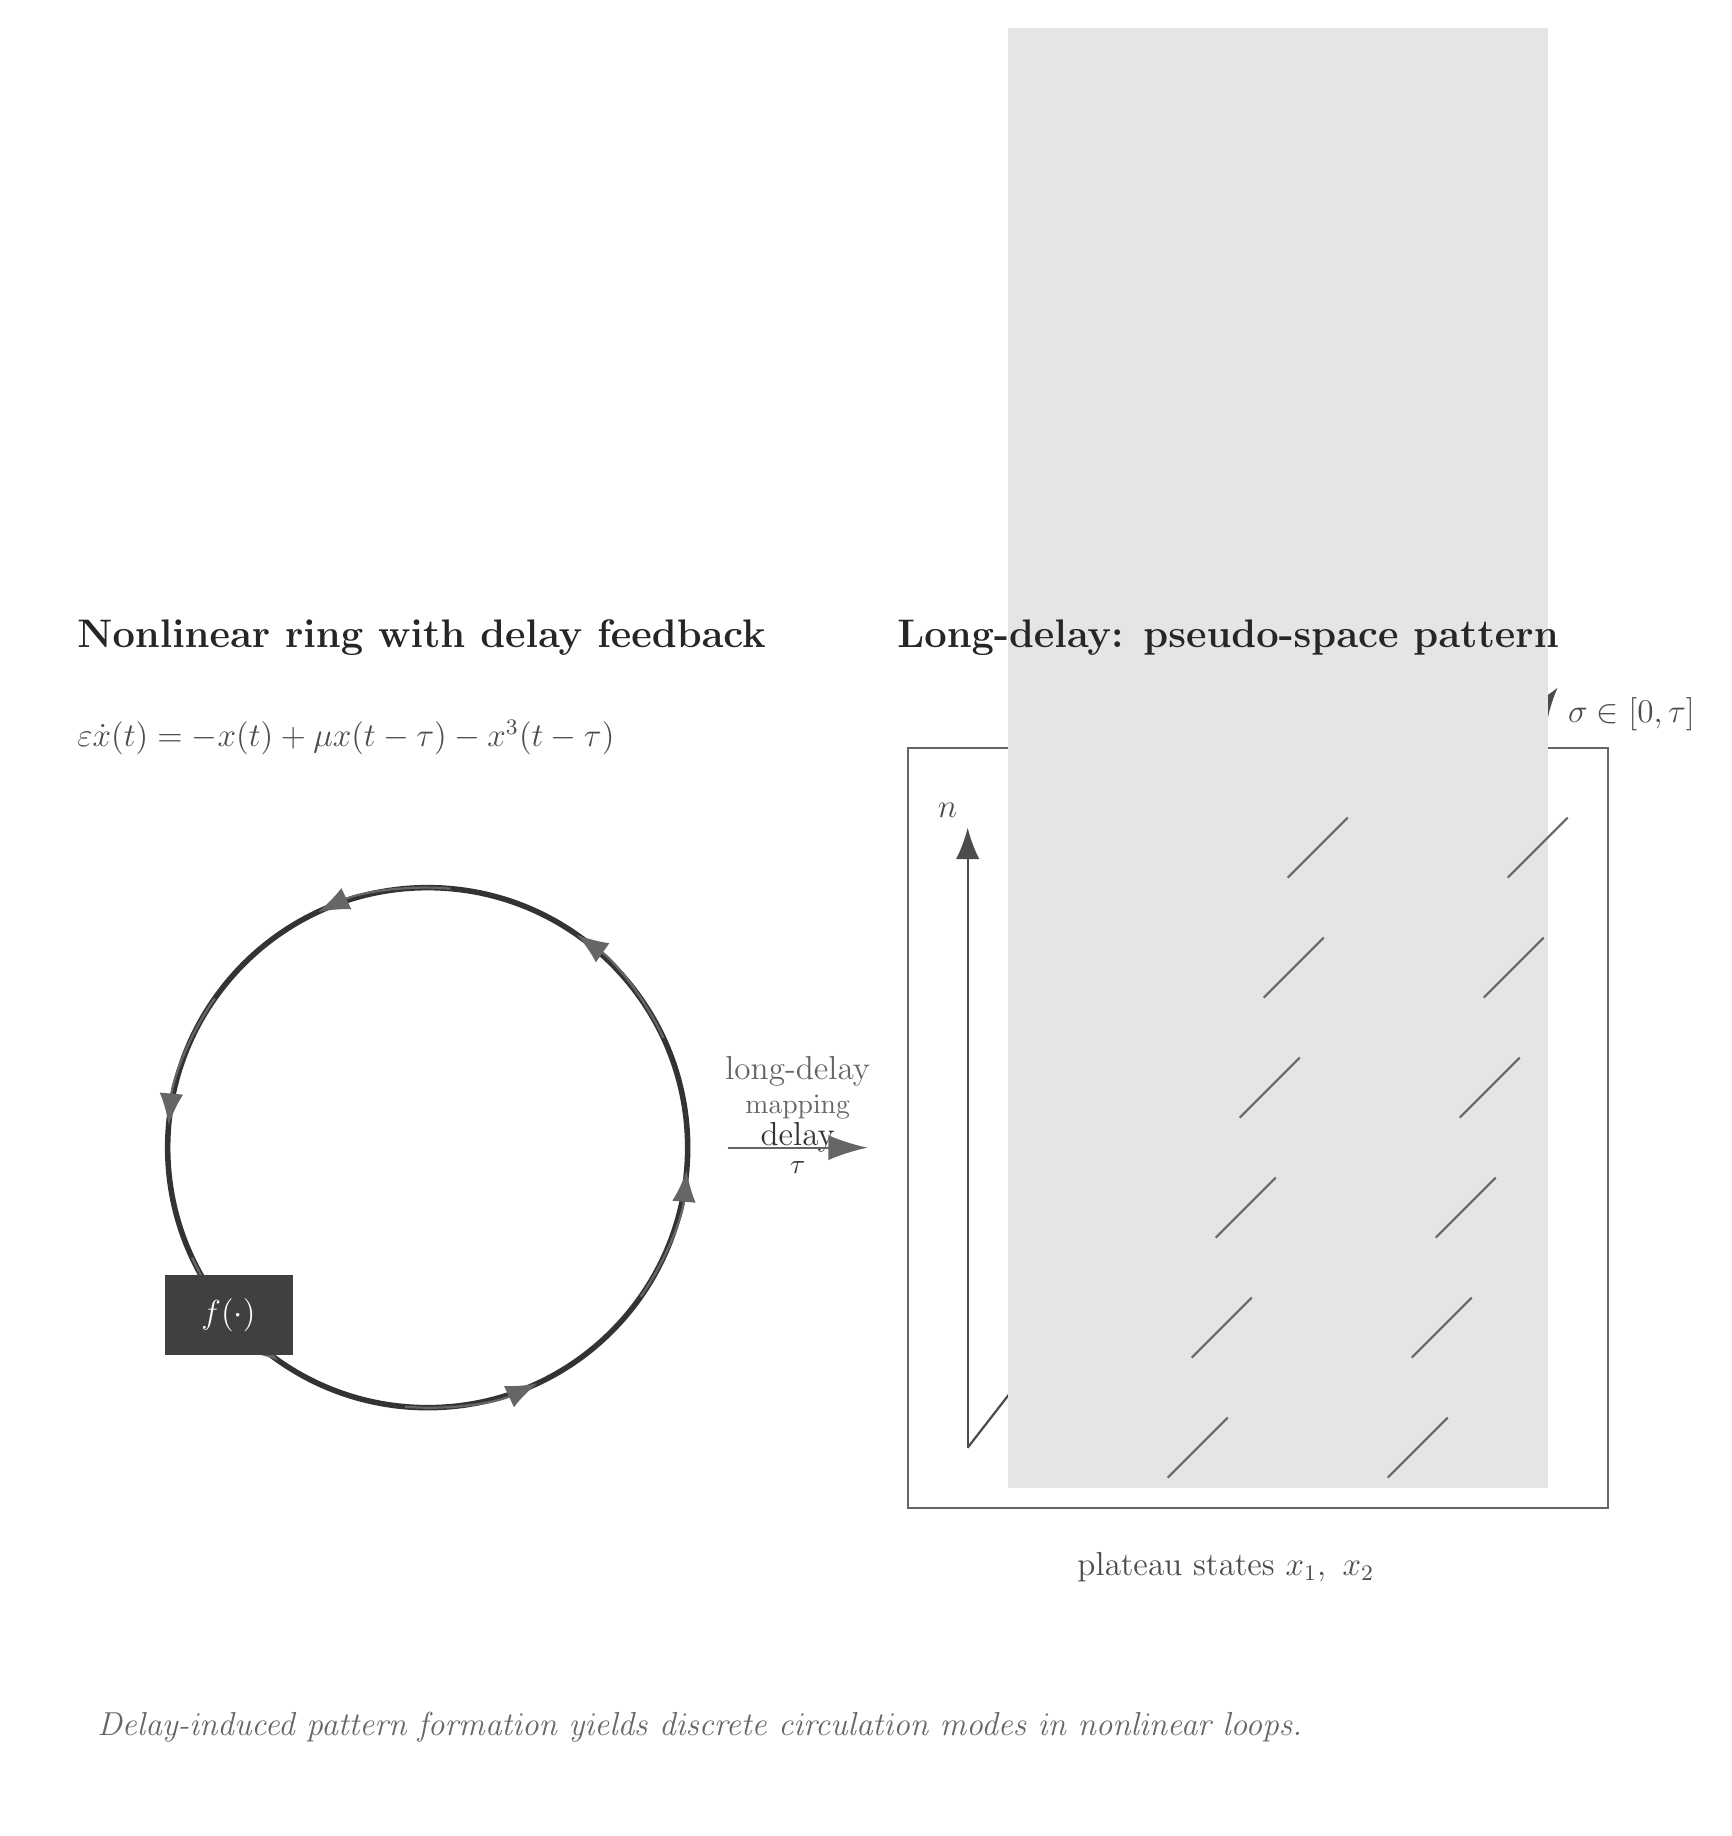
\begin{tikzpicture}[x=1in, y=1in]

% -- White Background --
        \fill[white] (0,0) rectangle (8.0139,6.2739);

% -- LEFT: Ring System --
        \coordinate (C) at (2.0,3.3);
        \def\R{1.3}
        \draw[line width=2pt, black!80] (C) circle (\R);

% Ring Arrows
        \foreach \a in {25,85,...,325} {
            \draw[-{Latex[length=4mm]}, black!60, thick]
            ($(C)+(\a:\R)$) arc[start angle=\a, end angle=\a+30, radius=\R];
        }

% Nonlinearity box
        \coordinate (NL) at ($(C)+(220:\R)$);
        \fill[black!75] ($(NL)+(-0.32,-0.2)$) rectangle ($(NL)+(0.32,0.2)$);
        \node[text=white] at (NL) {\large $f(\cdot)$};

% Delay label
        \node[align=center, text=black!80] at ($(C)+(0:\R+0.55)$) {\large delay\\[-2pt]$\tau$};

% Left labels
        \node[anchor=west, text=black!85] at (0.2,5.85)
            {\Large \textbf{Nonlinear ring with delay feedback}};
        \node[anchor=west, text=black!70] at (0.2,5.35)
            {\large $\varepsilon \dot{x}(t) = -x(t) + \mu x(t-\tau) - x^3(t-\tau)$};

% -- CONNECTOR --
        \draw[-{Latex[length=5mm,width=3.2mm]}, black!60, thick] (3.5,3.3) -- (4.2,3.3);
        \node[align=center, text=black!60] at (3.85,3.6) {\large long-delay\\mapping};

% -- RIGHT: Pseudo-space pattern --
        \coordinate (PBL) at (4.4,1.5);
        \coordinate (PTR) at (7.9,5.3);
        \draw[fill=white, draw=black!60, thick] (PBL) rectangle (PTR);

% Axes
        \draw[-{Latex[length=4mm]}, black!70, thick]
        ($(PBL)+(0.3,0.3)$) -- ($(PTR)+(-0.25,0.3)$)
        node[below right] {\large $\sigma \in [0,\tau]$};

        \draw[-{Latex[length=4mm]}, black!70, thick]
        ($(PBL)+(0.3,0.3)$) -- ($(PBL)+(0.3,3.4)$)
        node[above left] {\large $n$};

% Pattern plateaus
        \foreach \i in {0,...,8} {
            \pgfmathsetmacro{\yy}{1.6 + \i*0.4}
            \fill[black!10] ($(PBL)+(0.5,\yy-1.5)$) rectangle ($(PTR)+(-0.3,\yy-1.2)$);
        }

% Drifting fronts
        \foreach \i in {0,...,5} {
            \pgfmathsetmacro{\y}{1.65 + \i*0.6}
            \pgfmathsetmacro{\s}{0.12*\i}
            \draw[thick, black!60]
            ($(PBL)+(1.3+\s,\y-1.5)$) -- ($(PBL)+(1.6+\s,\y-1.2)$);
            \draw[thick, black!60]
            ($(PBL)+(2.4+\s,\y-1.5)$) -- ($(PBL)+(2.7+\s,\y-1.2)$);
        }

        \node[anchor=west, text=black!85] at (4.3,5.85)
            {\Large \textbf{Long-delay: pseudo-space pattern}};
        \node[anchor=west, text=black!70] at (5.2,1.2)
            {\large plateau states $x_1,\ x_2$};

% -- FOOTER --
        \node[anchor=west, text=black!60] at (0.3,0.4)
            {\large \textit{Delay-induced pattern formation yields discrete circulation modes in nonlinear loops.}};

    \end{tikzpicture}
\end{document}